\documentclass{article}
\usepackage[landscape]{geometry}
\usepackage{url}
\usepackage{multicol}
\usepackage{amsmath}
\usepackage{esint}
\usepackage{amsfonts}
\usepackage{tikz}
\usetikzlibrary{decorations.pathmorphing}
\usepackage{amsmath,amssymb}
\usepackage{pgfplots}


\usepackage{colortbl}
\usepackage{xcolor}
\usepackage{mathtools}
\usepackage{amsmath,amssymb}
\usepackage{enumitem}
\usepackage{hyperref}
\makeatletter

\newcommand{\N}{\mathbb{N}}
\newcommand{\Z}{\mathbb{Z}}
\newcommand{\Q}{\mathbb{Q}}
\newcommand{\R}{\mathbb{R}}
\newcommand{\C}{\mathbb{C}}
\newcommand{\K}{\mathbb{K}}
\newcommand{\m}{\cdot}
\newcommand{\vect}[1]{\mathbf{#1}} 

\newcommand*\bigcdot{\mathpalette\bigcdot@{.5}}
\newcommand*\bigcdot@[2]{\mathbin{\vcenter{\hbox{\scalebox{#2}{$\m@th#1\bullet$}}}}}
\makeatother

\title{Analysis 2 Cheat Sheet}
\usepackage[brazilian]{babel}
\usepackage[utf8]{inputenc}

\advance\topmargin-.8in
\advance\textheight3in
\advance\textwidth3in
\advance\oddsidemargin-1.5in
\advance\evensidemargin-1.5in
\parindent0pt
\parskip2pt
\newcommand{\hr}{\centerline{\rule{3.5in}{1pt}}}
%\colorbox[HTML]{e4e4e4}{\makebox[\textwidth-2\fboxsep][l]{texto}
\begin{document}


\begin{multicols*}{3}

\tikzstyle{mybox} = [draw=black, fill=white, very thick,
    rectangle, rounded corners, inner sep=10pt, inner ysep=10pt]
\tikzstyle{fancytitle} =[fill=black, text=white, font=\bfseries]


Sei im folgenden $A \subseteq \R^n$ und $\vect x^0 \in A$.\newline
%------------ Partielle Ableitungen allgemein---------------
\begin{tikzpicture}
\node [mybox] (box){%
    \begin{minipage}{0.3\textwidth}
    Sei $f:A \to \K$ und $j \in \{1,\dots,n\}$. Existiert ein $\varepsilon > 0$, s.d. $\forall h \in (-\varepsilon, \varepsilon): \vect x^0 + h\vect e_j \in A$, so nennen wir $f$ \textcolor{red}{in $\vect x^0$ partiell differenzierbar nach $x_j$}, wenn der Grenzwert $\lim \limits_{h \to 0} \frac{f(\vect x^0 + h\vect e_j) - f(\vect x^0)}{h}$ existiert.\\
    Den Grenzwert nennen wir dann \textcolor{red}{$j$-te partielle Ableitung von $f$ in $\vect x^0$} und wird bezeichnet durch: $\partial_j f(\vect x^0)$, $\partial_{x_j} f(\vect x^0)$, $\frac{\partial f(\vect x^0)}{\partial x_j}$, $f_{x_j}(\vect x^0)$, $D_jf(\vect x^0)$\\
    Randnotiz: Für $\vect x^0 \in \partial A$ definieren wir $\partial_j f(\vect x^0)$ so wie oben, bloss mit $h \in [0, \varepsilon)$ bzw. $h \in (\varepsilon, 0]$.\\
    \\
    Existieren alle partiellen Ableitungen von $f$ in $\vect x^0$, so nennen wir den (Zeilen)vektor $\nabla f(\vect x^0) = (\partial_1 f(\vect x^0),\dots, \partial_n f(\vect x^0))$ \textcolor{red}{Gradient von $f$ in $\vect x^0$}.\\
    \\
    Exisitert $\partial_j f(\vect x^0)$ für alle $\vect x^0 \in A$, so nennen wir die Funktion $\partial_j f: A \to \K, \vect x \mapsto \partial_j f(\vect x)$ die \textcolor{red}{$j$-te partielle Ableitung von $f$}.
    
    \end{minipage}
};


%------------ Partielle Ableitungen Header ---------------------
\node[fancytitle, right=10pt] at (box.north west) {Partielle Ableitungen von $f:\R^n \to \K$};
\end{tikzpicture}

%------------ Partielle Ableitung berechnen ---------------
\begin{tikzpicture}
\node [mybox] (box){%
    \begin{minipage}{0.3\textwidth}
    Um die $\partial_jf(\vect x^0)$ zu berechnen, falls diese existiert, tun wir so, als seien alle $x_i$ mit $i\neq j$ konstant und berechnen die Ableitung der Funktion\\ $\phi(x) := f(x_1^0, \dots, x_{j-1}^0, x, x_{j+1}^0, \dots, x_n^0)$ in $x = x_j^0$ wie im 1-dimensionalen Fall.
    \\
    Beispiel:\\
    Sei $f:\R^2\to \R, f(x_1,x_2) = x_1^2x_2 e^{2x_1+x_2} - 3x_2 + x_1$ und $\vect x^0 = (1,0)$. Dann ist\\
    $\partial_1f(x_1,x_2) = 2x_1x_2e^{2x_1+x_2}+2x_1^2x_2e^{2x_1+x_2} + 1$\\
    $\partial_2f(x_1,x_2) = x_1^2e^{2x_1+x_2}+x_1^2x_2e^{2x_1+x_2} - 3$\\
    $\nabla f(\vect x^0) = (1, e^2-3)$
    \end{minipage}
};

%------------ Partielle Ableitung berechnen Header ---------------------
\node[fill=purple, text=white, font=\bfseries, right=10pt] at (box.north west) {Partielle Ableitung berechnen};
\end{tikzpicture}



%------------ Jacobimatrix ---------------
\begin{tikzpicture}
\node [mybox] (box){%
    \begin{minipage}{0.3\textwidth}
    Sei $f:A \to \K^m$. Existieren alle partiellen Ableitungen $\partial_jf_l(\vect x^0)$ für $j\in \{1,\dots,n\}, l\in \{1,\dots,m\}$, dann nennen wir die $m \times n$-Matrix\\
    $\begin{bmatrix} \partial_1 f_1(\vect x^0) & \dots & \partial_n f_1(\vect x^0)\\ \vdots &  & \vdots \\ \partial_1 f_m(\vect x^0)& \dots & \partial_n f_m(\vect x^0)\end{bmatrix}=\begin{bmatrix} \nabla f_1(\vect x^0) \\ \vdots \\ \nabla f_m(\vect x^0) \end{bmatrix}$\\die \textcolor{red}{Jacobimatrix von $f$ in $\vect x^0$} und bezeichnen diese mit \textcolor{red}{$J_f(\vect x^0)$}. Für $m=n$ bezeichnen wir $\det(J_f(\vect x^0))$ als die \textcolor{red}{Jacobideterminante von $f$ in $\vect x^0$}.

    
    \end{minipage}
};

%------------ Jacobimatrix Header ---------------------
\node[fancytitle, right=10pt] at (box.north west) {Partielle Ableitungen von $f:\R^n \to \K^m$};
\end{tikzpicture}


%------------ Partielle Ableitung Eigenschaften ---------------
\begin{tikzpicture}
\node [mybox] (box){%
    \begin{minipage}{0.3\textwidth}
    Die $j$-te partielle Ableitung ist eine lineare Funktion. Somit sind auch der Gradient und die Jacobimatrix lineare Funktionen.\\
    Das heißt $\forall \lambda \in \K, \forall l \in \{1,\dots, m\}, k \in \{1,\dots,n\}: $\\
    $\partial_j(\lambda f+g)_l(\vect x^0) = \lambda \cdot \partial_j(f)_l(\vect x^0) + \partial_j(g)_l(\vect x^0)$\\
    $\nabla(\lambda f+g)_l(\vect x^0) = \lambda \cdot \nabla f_l(\vect x^0) + \nabla g_l(\vect x^0)$\\
    $J_{\lambda f+g}(\vect x^0) = \lambda \cdot J_f(\vect x^0) + J_g(\vect x^0)$
    \end{minipage}
};

%------------ Partielle Ableitung Eigenschaften Header ---------------------
\node[fill=blue, text=white, font=\bfseries, right=10pt] at (box.north west) {Eigenschaften von partiellen Ableitungen};
\end{tikzpicture}


%------------ Jacobimatrix Beispiel ---------------
\begin{tikzpicture}
\node [mybox] (box){%
    \begin{minipage}{0.3\textwidth}
    Die Funktion $f:\R^3 \to \R^2$ sei gegeben durch $f(x_1,x_2,x_3) = \begin{pmatrix} x_1^2 + x_2^2\\ x_3^2 + x_3\cdot \sin(x_2) \\ x_2x_3 \end{pmatrix}$\\
    $\partial_1f(x_1,x_2,x_3) = \begin{pmatrix} 2x_1\\ 0 \\ 0\end{pmatrix}$\\
    $\partial_2f(x_1,x_2,x_3) = \begin{pmatrix} 2x_2^2 \\ x_3\cdot \cos(x_2)\\ x_3\end{pmatrix}$\\
    $\partial_3f(x_1,x_2,x_3) = \begin{pmatrix} 0 \\ 2x_3 +\sin(x_2)\\ x_2\end{pmatrix}$\\
    $J_f(x_1,x_2,x_3) = \begin{pmatrix} 2x_1 &  2x_2^2 & 0\\ 0 & x_3\cdot \cos(x_2) & 2x_3 +\sin(x_2) \\ 0 & x_3 & x_2\end{pmatrix}$\\
    $J_f(1,0,1) = \begin{pmatrix} 2 &  0 & 0\\ 0 & 1 & 2 \\ 0 & 1 & 0\end{pmatrix}, \det(J_f(1,0,1)) = -4$. 
    \end{minipage}
};

%------------ Jacobimatrix Beispiel Header ---------------------
\node[fill=purple, text=white, font=\bfseries, right=10pt] at (box.north west) {Jacobimatrix Beispiel};
\end{tikzpicture}


%------------ Partielle Ableitungen höherer Ordnung Beispiel ---------------
\begin{tikzpicture}
\node [mybox] (box){%
    \begin{minipage}{0.3\textwidth}
    Sei $f:A \to \K^m$ und $k \in \N$.\\ Für jedes $p = (p_1,\dots,p_k) \in \{1,\dots,n\}^k$ nennen wir\\
    $\partial_pf(\vect x^0) := \frac{\partial^kf(\vect x^0)}{\partial x_{p_1} \dots \partial x_{p_k}} := \partial_{p_1} \partial_{p_2} \dots \partial_{p_k} f(\vect x^0)$\\
    die \textcolor{red}{partielle Ableitung $k$-ter Ordnung von $f$ in $\vect x^0$ nach $p$} (wenn existent). D.h. wir berechnen zuerst die $p_k$-te partielle Ableitung von $f$, dann davon die $p_{k-1}$-te partielle Ableitung, usw. und zum Schluss die $p_1$-te partielle Ableitung.\\
    $f$ selbst wird auch als partielle Ableitung $0$-ter Ordnung bezeichnet.\\
    \end{minipage}
};

%------------ Partielle Ableitungen höherer Ordnung Header ---------------------
\node[fill=black, text=white, font=\bfseries, right=10pt] at (box.north west) {Partielle Ableitungen höherer Ordnung};
\end{tikzpicture}


%------------ Jacobideterminante Idee ---------------
\begin{tikzpicture}
\node [mybox] (box){%
    \begin{minipage}{0.3\textwidth}
    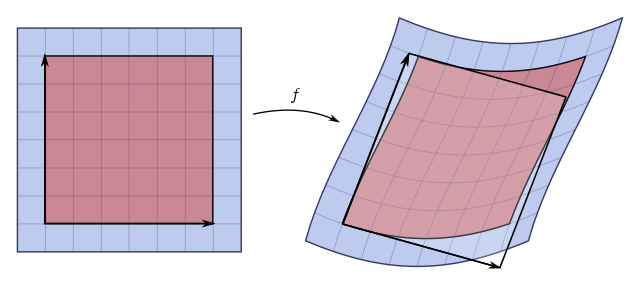
\includegraphics[scale = .35]{Jacobian_determinant.png}
    Eine nicht-lineare Abbildung $f:\R^2\to\R^2$ transformiert ein Rechteck (links in rot) zu einer verzerrten Fläche (rechts in rot). Würden wir für das rote Rechteck die Funktionswerte mit Hilfe der Jacobimatrix linear approximieren, dann würden wir das rote Rechteck in das weiße durchsichtige Parallelprogramm überführen. Die Jacobideterminante ist das Verhältnis von der Fläche des ursprünglichen Rechtecks zum weißen durchsichtigen Parallelprogramm und dient, in der Umgebung von dem Punkt in dem wir sie berechnet haben, als Approximation für das Verhältnis von der Fläche des ursprünglichen Rechtecks zur verzerrten roten Fläche.
    \end{minipage}
};

%------------ Jacobideterminante Idee Header ---------------------
\node[fill=purple, text=white, font=\bfseries, right=10pt] at (box.north west) {Idee der Jacobideterminante};
\end{tikzpicture}

%------------ Satz von Schwarz ---------------
\begin{tikzpicture}
\node [mybox] (box){%
    \begin{minipage}{0.3\textwidth}
    Sei $f:A \to \K$. Sind alle partiellen Ableitungen 2-ter Ordnung von $f$ in $\vect x^0$ stetig, dann gilt:\\ $\forall i,j \in \{1,\dots,n\}: \partial_i \partial_j f(\vect x^0) = \partial_j \partial_i f(\vect x^0)$
    
    
    \end{minipage}
};

%------------ Satz von Schwarz Header ---------------------
\node[fill=blue, text=white, font=\bfseries, right=10pt] at (box.north west) {Satz von Schwarz};
\end{tikzpicture}

%------------ C^k Raum ---------------
\begin{tikzpicture}
\node [mybox] (box){%
    \begin{minipage}{0.3\textwidth}
    Sei $f:A \to \K^m$ und $k \in \N_0$. Wir nennen $f$ eine \textcolor{red}{$C^k$-Funktion}, wenn für alle Koordinatenfunktionen $f_l$ alle partiellen Ableitungen der Ordnung 0 bis $k$ von $f_l$ in $A$ existieren und stetig sind.\\
    Die Menge aller $\K^m$-wertigen $C^k$-Funktionen auf $A$ bezeichnen wir mit $C^k(A,\K^m)$.\\
    Haben alle $f_l$ stetige partielle Ableitungen beliebiger Ordnung, so nennen wir $f$ eine \textcolor{red}{$C^\infty$-Funktion} oder \textcolor{red}{glatte Funktion}.
    
    \end{minipage}
};

%------------ C^k Raum Header ---------------------
\node[fill=black, text=white, font=\bfseries, right=10pt] at (box.north west) {$C^k$-Funktionen};
\end{tikzpicture}

\newpage

%------------ Totales Differential ---------------
\begin{tikzpicture}
\node [mybox] (box){%
    \begin{minipage}{0.3\textwidth}
    Sei $A$ offen und $f:A \to \R^m$ und $k \in \N_0$. Wir nennen $f$ \textcolor{red}{differenzierbar in $\vect x^0$}, wenn eine lineare Abbildung $L_{\vect x^0}: \R^n \to \R^m$ existiert, so dass\\
    $\lim \limits_{\vect h \to 0} \frac{f(\vect x^0 + \vect h) - f(\vect x^0) - L_{\vect x^0}(\vect h)}{\Vert \vect h \Vert} = \vect 0$\\
    Ist $f$ differenzierbar in $\vect x^0$, so nennen wir $L$ das \textcolor{red}{totales Differential} oder \textcolor{red}{totale Ableitung von $f$ in $\vect x^0$} und wir schreiben dann $Df(\vect x^0)$ statt $L$.
    \end{minipage}
};

%------------ Totales Differential Header ---------------------
\node[fill=black, text=white, font=\bfseries, right=10pt] at (box.north west) {Totales Differential/ Totale Ableitung};
\end{tikzpicture}



%------------ Totales Differential Intuition ---------------
\begin{tikzpicture}
\node [mybox] (box){%
    \begin{minipage}{0.3\textwidth}
    Im eindimensionalen haben wir die Ableitung bestimmt, indem wir zwischen $f(x^0)$ und $f(x^0 + h)$ eine Linie/Gerade (lineare Funktion)  zeichnen und davon die Steigung bestimmen. Die Ableitung ist dann diese Steigung für $h \to 0$. 
    Im mehrdimensionalen reicht eine Gerade dafür nicht mehr aus, da es nun unendlich viele Punkte um $\vect x^0$ gibt, die Abstand $\Vert \vect h \Vert$ zu $\vect x^0$ haben. Das heißt wir brauchen eine Verallgemeinerung von "Linie"/"Gerade". Diese wäre im mehrdimensionalen eine lineare Abbildung $L$ für die gilt, dass für $\vect h \approx \vect 0$ gilt:
    $f(\vect x^0 + h) \approx f(\vect x^0) + L(\vect h)$.
    Von der linearen Abbildung $L$ können wir analog zu der Gerade im eindimensionalen die "Steigung"/Ableitung in alle Richtungen bestimmen. Wenn wir also den Grenzwert dazu bilden und dieser existiert, dann nennen wir diesen die totale Ableitung von $f$ in $\vect x^0$.\\
    Geometrisch bedeutet differenzierbar, so wie im eindimensionalen, dass $f$ keine Sprünge und keine Knicke hat. Bei einer mehrdimensionalen Funktion kann man sich "Knick" als Falte oder Zacken vorstellen. Die Existenz der partiellen Ableitungen bedeutet nur, dass es keine Knicke in Richtung der Achsen gibt. Dennoch kann es in eine andere Richtung betrachtet Knicke geben. Deswegen folgt aus der Existenz der partiellen Ableitungen in $\vect x^0$ \textbf{nicht}, dass $f$ in $\vect x^0$ differenzierbar ist.
    
    \end{minipage}
};

%------------ Totales Differential Intuition Header ------------------
\node[fill=purple, text=white, font=\bfseries, right=10pt] at (box.north west) {Idee/Intuition Totales Differential};
\end{tikzpicture}


%------------ Totales Differential Satz ---------------
\begin{tikzpicture}
\node [mybox] (box){%
    \begin{minipage}{0.3\textwidth}
    Sei $f:A \to \K^m$ differenzierbar in $\vect x^0$. Dann ist $f$ stetig in $\vect x^0$, alle $\partial_k f_l(\vect x^0)$ existieren und es gilt $Df(\vect x^0) = J_f(\vect x^0)$.
    Im Fall von $m = 1$ gilt dann also $Df(\vect x^0) = \nabla f(\vect x^0)$
    \end{minipage}
};

%------------ Totales Differential Satz Header ------------------
\node[fill=blue, text=white, font=\bfseries, right=10pt] at (box.north west) {Totales Differential Satz};
\end{tikzpicture}


%------------ Totales Differential Satz ---------------
\begin{tikzpicture}
\node [mybox] (box){%
    \begin{minipage}{0.3\textwidth}
    Sei $f:A \to \K^m$. Existieren alle $\partial_jf_l$ auf ganz $A$ und sind diese stetig in $\vect x^0$, so ist $f$ differenzierbar in $\vect x^0$.
    \end{minipage}
};

%------------ Totales Differential Satz Header ------------------
\node[fill=blue, text=white, font=\bfseries, right=10pt] at (box.north west) {Totales Differential Satz};
\end{tikzpicture}

%------------ Kettenregel ---------------
\begin{tikzpicture}
\node [mybox] (box){%
    \begin{minipage}{0.3\textwidth}
    Sei $A_f \subseteq \R^n$ offen und $f: A_f \to \R^m$. \\Sei $f(A_f) \subseteq A_g \subseteq \R^m$ offen und $g: A_g \to \K^p$. Ist $f$ differenzierbar in $\vect x^0$ und $g$ differenzierbar in $f(\vect x^0)$, so ist $g \circ f:A_f \to \K^p$ differenzierbar in $\vect x^0$ und es gilt die Kettenregel:\\
    $D(g\circ f)(\vect x^0) = Dg(f\vect x^0)) \circ Df(\vect x^0)$\\
    Insbesondere gilt, wenn $f$ und $g$ differenzierbar sind, so ist auch $g \circ f$ differenzierbar.
    \end{minipage}
};

%------------ Kettenregel Header ------------------
\node[fill=blue, text=white, font=\bfseries, right=10pt] at (box.north west) {Kettenregel};
\end{tikzpicture}

%------------ Weg-zusammenhängend ---------------
\begin{tikzpicture}
\node [mybox] (box){%
    \begin{minipage}{0.3\textwidth}
    Wir nennen $A$ \textcolor{red}{weg-zusammenhängend}, wenn für alle $\vect x, \vect y \in A$ eine stetige Funktion $p:[0,1] \to A$ existiert mit $p(0) = x$ und $p(1) = y$.\\Ist $p$ auch noch differenzierbar, dann nennen wir $A$ differenzierbar weg-zusammenhängend.
    \end{minipage}
};

%------------ Weg-zusammenhängend Header ------------------
\node[fill=black, text=white, font=\bfseries, right=10pt] at (box.north west) {Weg-zusammenhängend};
\end{tikzpicture}


%------------ Weg-zusammenhängend Beispiel---------------
\begin{tikzpicture}
\node [mybox] (box){%
    \begin{minipage}{0.3\textwidth}
    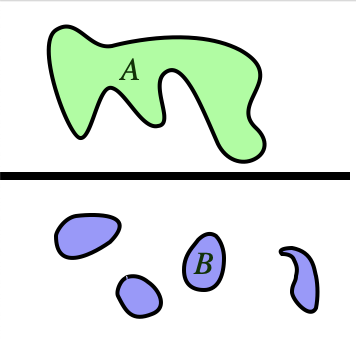
\includegraphics[scale = .75]{path_conn.png}\\ Die Menge A ist weg-zusammenhängend, weil du alle Punkte aus der Menge mit einem stetigen Pfad innerhalb der Menge verbinden kannst.
    Die Menge B ist nicht weg-zusammenhängend, da es keinen stetigen Pfad von einem Punkt aus der ersten "Bubble" zu einem Punkt in der letzten "Bubble" gibt.
    \end{minipage}
};

%------------ Wegzusammenhängend Beispiel Header ------------------
\node[fill=purple, text=white, font=\bfseries, right=10pt] at (box.north west) {Weg-zusammenhängend};
\end{tikzpicture}

%------------ Gradient gleich 0 Satz Beispiel---------------
\begin{tikzpicture}
\node [mybox] (box){%
    \begin{minipage}{0.3\textwidth}
    Ist $A$ differenzierbar weg-zusammenhängend und \\$f:A \to \K$ differenzierbar mit $\nabla f \equiv 0$, dann ist $f$ konstant.
    \end{minipage}
};

%------------ Gradient gleich 0 Satz Header ------------------
\node[fill=blue, text=white, font=\bfseries, right=10pt] at (box.north west) {Konstante Funktion};
\end{tikzpicture}


%------------ Richtungsableitung ---------------
\begin{tikzpicture}
\node [mybox] (box){
    \begin{minipage}{0.3\textwidth}
    Sei $\vect r \in \R^n$ mit $\Vert \vect r \Vert = 1$ und sei $f$ stetig differenzierbar in $\vect x^0$, dann nennen wir $\frac{\partial f}{\partial \vect r}(\vect x^0) := \frac{df(\vect x^0 + t\cdot \vect r)}{dt}(0)$ \textcolor{red}{(erste) Richtungsableitung von $f$ in Richtung $\vect r$ an der Stelle $\vect x^0$}.
    \end{minipage}
};

%------------ Richtungsableitung Header ------------------
\node[fill=black, text=white, font=\bfseries, right=10pt] at (box.north west) {Richtungsableitung};
\end{tikzpicture}


%------------ Richtungsableitung Satz Beispiel---------------
\begin{tikzpicture}
\node [mybox] (box){
    \begin{minipage}{0.3\textwidth}
    Sei $f:A \to \K$ differenzierbar in $\vect x^0$, so existieren für alle $\vect r \in R^n$ mit $\Vert \vect r \Vert = 1$ die Richtungsableitung $\frac{\partial f}{\partial \vect r}(\vect x^0)$ und es gilt
    $\frac{\partial f}{\partial \vect r}(\vect x^0) = \nabla f(\vect x^0) \cdot \vect r$\\
    \\
    Die Richtung $\vect r = \frac{\nabla f(\vect x^0)}{\Vert \nabla f(\vect x^0) \Vert}_2$ ist die Richtung des steilsten Anstiegs an der Stelle $\vect x^0$.
    \end{minipage}
};

%------------ Richtungsableitung Satz Header ------------------
\node[fill=blue, text=white, font=\bfseries, right=10pt] at (box.north west) {Richtungsableitung Satz};
\end{tikzpicture}

\end{multicols*}

\end{document}